% 105-25(105쪽) — 함수 y=f(x) 의 그래프(꺾인점 (-2,0) 에서 만나는 직선 2개). 스캔 화질이 낮아 TikZ 로 다시 그림.
% 원문에 있는 것만: 눈금 숫자 −3 −2 (x) · 2 1 (y, 축 오른쪽) · 라벨 O, x, y, y=f(x) · (-3,2) 로 가는 안내 파선.
% 왼쪽 직선은 (-3,2) 와 (-2,0) 을, 오른쪽 직선은 (-2,0) 과 y절편 1 을 지난다 — 원문 그림에서 잰 자리 그대로다.
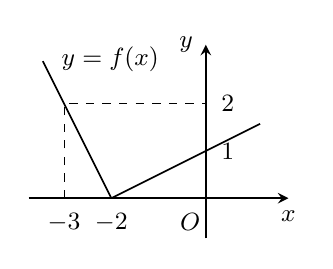
\begin{tikzpicture}[x=0.60cm, y=0.60cm, line width=0.5pt]
  \draw[->, >=stealth, line width=0.7pt] (-3.75,0) -- (1.75,0) node[below=1pt, font=\small] {$x$};
  \draw[->, >=stealth, line width=0.7pt] (0,-0.85) -- (0,3.25) node[left=1pt, font=\small] {$y$};
  \node[below=2pt, font=\small] at (-0.33,0) {$\pt{O}$};
  % 좌표 안내 파선(원문)
  \draw[dashed, line width=0.35pt] (-3,0) -- (-3,2) -- (0,2);
  % 그래프
  \draw[line width=0.6pt] (-3.45,2.9) -- (-2,0);
  \draw[line width=0.6pt] (-2,0) -- (1.15,1.575);
  % 눈금 라벨(원문 자리 그대로: y 눈금 2·1 은 축 오른쪽)
  \node[right=2pt, font=\small] at (0,2) {$2$};
  \node[right=2pt, font=\small] at (0,1) {$1$};
  \node[below=2pt, font=\small] at (-3,0) {$-3$};
  \node[below=2pt, font=\small] at (-2,0) {$-2$};
  \node[right=1pt, font=\small] at (-3.32,2.95) {$y=f(x)$};
\end{tikzpicture}
